\documentclass{article}

\usepackage{mathtools}
\usepackage{amssymb}
\usepackage{cancel}
\usepackage{tcolorbox}
\usepackage{fancyhdr}
\usepackage{tikz}
\usepackage[margin=1in]{geometry}

\pagestyle{fancy}
\everymath{\displaystyle}

\title{FCA}
\author{ale-cci}

\begin{document}
\maketitle
\newpage
\section{Lezione 8 - Stabilit\'a dei sistemi dinamici}
Un sistema lineare $\sum$ si dice:
\begin{enumerate}
    \item STABILE se per ogni perturbazione $y_{lib}(t)$ \'e limitata su $[0,+\infty)$

        $\sum$ \'e stabile $\Leftrightarrow$ tutti i poli hanno parte reale non positiva e gli eventuali poli puramente immaginari sono semplici
    \item ASINTOTICAMENTE STABILE, se stabile e $lim_{t \to+\infty} y_{lib}(t) = 0$A per ogni perturbazione introdotta.
    \item SEMPLICEMENTE STABILE \'e stabile ed esiste una perturbazione  per cui

    \[ \lim_{t \to +\infty} y_{lib}(t) = y_{\infty} \neq 0 \lor \big\{\text{Non esiste $lim_{t\to\infty} y_{lib}(t)$}\big\} \]
    \item INSTABILE non \'e stabile
\end{enumerate}

\newpage
\section{Trasformata Z}
Dato un segnale a tempo discreto ($x(k) : \mathbb{Z} \to \mathbb{C}$), La trasformata zeta di $x(k)$ \`e definita come:
\[ \mathcal{Z}[x] \coloneqq \sum\limits^{+\infty}_{k=0} x(k) z^{-k}\]

\textit{Es:}
$ \mathcal{Z}[\delta(k)] = \sum\limits_{k=0}^{+\infty} \delta{k}z^{-k} = 1 $

La trasformata $\mathcal{Z}$ \`e lineare:
$ \mathcal{Z}[ax(k) + by(k)] = a\mathcal{Z}[x(k)] + b\mathcal{Z}[y(k)] $\\

Per calcolare $\mathcal{Z}[\sin(\omega k)]$ e $\mathcal{Z}[\sin(\omega k)]$, basta $\mathcal{Z}[e^{i\omega k}]$, poi utilizzare la formula per serie geometrica di regione $q < 1$: $\sum\limits_{k=0}^{+\infty} q^k = \frac{1}{1-q} $, ottenendo:

\[ \mathcal{Z}[\sin (\omega k)] = \frac{z\sin\omega}{z^2 - 2z\cos \omega +1} \]
\[ \mathcal{Z}[\cos (\omega k)] = \frac{z(z - \cos\omega)}{z^2 - 2z\cos \omega +1} \]

\subsection{Propiet\'a trasformata Z}
Trasformata di un segnale in ritardo di $n$ passi:
\[ \mathcal{Z}[x(k-n)] = z^{-n}\mathcal{Z}[x(k)] + \sum\limits_{k=0}^{n-1} x(k-n) z^{-k} \]

Segnale anticipato di $n$ passi:
\[ \mathcal{Z}[x(k+n)] = z^n\mathcal[x(k)] - \sum\limits_{k=0}^{n-1}x(k)z^{n-k} \]

Teorema valore iniziale: $x(0) = \lim\limits_{z\to +\infty} \mathcal{Z}[x(k)] $

Teorema valore finale (valido solo se $x(k)$ \`e limitata):
$\lim\limits_{k\to +\infty} x(k) = \lim\limits_{z \to 1} (z-1) \mathcal{Z}[x(k)] $

Trasformata di $a^kx(k)$: $X(z')\Big|_{z'=\frac{z}{a}}$

Derivata trasformata Z: $\mathcal{Z}[k\cdot x(k)] = -z \frac{dX(z)}{dz}$

Trasformata gradino: $\mathcal{Z}[1(k)] = \frac{z}{z-1} $

Trasformata convoluzione: $\mathcal{Z}[x(k) \ast y(k)] = X(z)\cdot Y(z)$

\section {Antitrasformazione Zeta}
\[ x(k) = \sum\limits_i Res\{ X(z) z^{k-1}, P_i \} \]

Antitrasformate Notevoli:
\[ \mathcal{Z}^{-1}\left[ \frac{c}{z-p} + \frac{\bar c}{z-p} \right] = 2|c||p|^{k-1} \cos((k-1) \arg p + \arg c )\, 1(k-1) \]
\[ \mathcal{Z}^{-1}\left[ \frac{1}{z-a}\right] = a^{k-1} \cdot 1(k-1) \]

\section{Criterio di Juri}
Sia dato il polinomio $a(z) = a_n z^n + a_{n-1} z^{n-1} + \cdots + a_n$ con $a_n > 0$. Condizione necessaria affich\'e $a(z)$ abbia tutte le radici di modulo minore di $1$ \'e che le seguenti disuguaglianze siano soddisfatte:

\begin{enumerate}
    \item $a(1) > 0$
    \item $(-1)^n a(-1) > 0$
    \item $|a_0| < a_n$
\end{enumerate}

Perndendo come esempio il caso $n - 1$:
\[ a(z) = a_1z + a_0 = 0 \]
\[ z = -\frac{a_0}{a_1} \qquad |z| < 1 \quad \Leftrightarrow \quad \frac{|a_o|}{a_1} < 1 \quad \Leftrightarrow\quad  \framebox{$|a_o| < a_1$} \]

Otteniamo che:
\begin{itemize}
    \item $ a(1) = a_1 + a_0 > 0$
    \item $ a(-1) = -a_1 + a_0 < 0$
\end{itemize}

di queste tre disuguaglianze solo 2 sono indipendenti: la terza \'e l'insieme della prima e della seconda

Per il caso $n = 2$: 3 condizioni distinte (page 14 di Lez. 21)


\bigbreak
Anche nel criterio di Jury \'e necessario costruire una trabella: (slide 15 Lez 21)
\begin{itemize}
    \item iniziamo a scrivere le prime due righe: con la prima riga iniziamo a scrivere a partire da $a_0$
    \item Per la seconda riga partiamo da $a_n$ e terminiamo la riga a $a_0$
    \item Per costruire le right successive calcoliamo il determinante della matrice $2\times 2$ sopra e riportiamo la stessa riga sotto al contrario
\end{itemize}

Per calcolare il termine di una determinata riga si utilizza la formula:
\[
    b_k = \det\begin{pmatrix}
        a_0 & a_{n-k}\\
        a_n & a_k
    \end{pmatrix} \quad k = 0,1\ldots n-1
\]

\section{Teorema (criterio di Jury)}
Il polinomio $a(z) = \ldots$ ha tutte le radici di modulo minore di 1 se e solo se le seguenti $n+1$ disuguaglianze sono soddisfatte:
\begin{enumerate}
    \item $a(1) > 0$
    \item $(-1)^n a(-1) > 0$
    \item $\ldots$ slide 16
\end{enumerate}

\section{Scelta del periodo di campionamento (Slide 18 Lez 21)}

Per il teorema di campionamento
\[ w_s > 2w_b \]
con $w_s = \frac{2\pi}{}$ pulsazione di campionamento, $T$ il corrispondente periodo

Una volta realizzato il progetto in tempo continuo \'e necessario implementare una $C_d(z)$

Alla funzione $C(s)$ \'e associata un'equazine differenziale in tempo continuo, a $C_d(z)$  un equazione di differenze

Metodo di eulero: $Dx(T) \Rightarrow \mathcal{L}[Dx(t)] = s\cdot\mathcal{L}[x(t)]$ (condizione iniziale nulla)
\[ Dx(kT) \approx \frac{x((k+1)T) - x(kT)}{T}\]
\[ \mathcal{Z}[Dx(kT)]  \approx \frac{z-1}{T}\mathcal{Z}[x(kT)]\]
\[ s = \frac{z-1}{Tz}\]

\subsubsection{Alla lavagna}

Immaginando di avere la funzione differenziale $a_1 Dy + a_0y = b_1Du + b_0u$ corrisponde una funzione di trasferimento.
Trasformandola secondo laplace con, condizioni iniziali nulle si ottiene:

\[ a_1 sY + a_0 Y = b_1 sU + b_0 U \]

Immaginandola in tempo discreto, imponendo $t = kT$
\[ a_1 Dy(kT) + a_0 y(kT_ = b_1 Du(kT) + b_0u(kT) \]

NOTA: Fino ad adesso Non \'e una approssimazione

Ora per calcolare la derivata utilizzo l'euqazione di eulero
\[ a_1 \frac{y((k+1)T) - y(kT)}{T} + a_0 y(kT) = b_1\frac{u((k+1)T) - u(kT)}{T} + b_0u(kT)\]

Trasformanso:
\[ \mathcal{Z}\left\{a_1 \frac{y((k+1)T) - y(kT)}{T} + a_0 y(kT) = b_1\frac{u((k+1)T) - u(kT)}{T} + b_0u(kT)\right\}\]

\[ \cdots\]
\[ a_1 \frac{z-1}{T} \mathcal{Z}[y(kT)] + a_0 \mathcal{Z}[y(kT)] = b_1 \frac{z-1}{T} \mathcal{Z}[u(kT)] + b_0 \mathcal{Z}[u(kT)]\]

Trovo cos\`i che:
\[ Y(z) = \frac{b_1\frac{z-1}{T} + b_0}{a_1\frac{z-1}{T} + a_0} U(z) = \left.C(s)\right|_{s=\frac{z-1}{T}} U(z) \coloneqq H(z)U(z)\]

\bigbreak

\textbf{Metodo di Euolero all'indietro}: Stimo la derivata guardando il campione precedente

\[ Dx(kT) \approx \frac{x(kT) - x((k-1)T)}{T}\]

\subsubsection{Metodo di Tustin (slide 21)}
Viene utilizzata l' `approssimazione col metodo del trapezio'

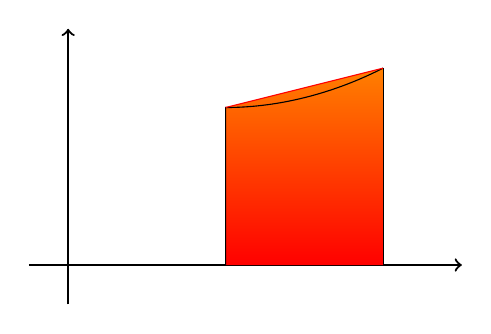
\begin{tikzpicture}
    \draw [thick, ->] (-0.5, 0) -- (5, 0);
    \draw [thick, ->] (0, -0.5) -- (0, 3);
    \shade[top color=orange, bottom color=red] (2, 2) -- (4, 2.5) |- (2, 0);
    \draw (2, 0) -- (2, 2)
            parabola (4, 2.5);
    \draw (4, 0) -- (4, 2.5);

    \draw [color = red] (2, 2) -- (4, 2.5);

\end{tikzpicture}

(x: Approssimare due  punti con trapezio)

Da slide 24: $C_d(z)$ \`e asintoticamente stabile siccome tutti i poli sono contenuti nella circonferenza unitaria






\newpage
\section{Esercizi}
\subsection{Ex Lez 20 Slide 16}

\subsubsection{Parte 1}

\[
    y_0(K+2) = y(K+1) - 0.24y(K) + u(K+2)\\
\]
\bigbreak
\(
    a_ny(K) + a_{N-1}y(K-1) + \cdots +a_o y(K-1) = b_n u(K-n +m) + b_{n-1} u(K-n+m-1) + \cdots + b_o u(K-n)
\)

\(
\Leftrightarrow H(z) = \frac{b_mz^{n} + b_{m-1}z^{m-1}+ \cdots + b_o}{a_mz^n + a_{n-1}z^{n-1}+a_0}
\)
\bigbreak

\(
\begin{cases}
a_n \neq 0\\
b_m \neq 0 \\
m \le n
a_0 \lor b_0 \neq 0
\end{cases}
\)

\[
\begin{split}
K \leftarrow K-1\\
y(K) = y(K-1) - 0.24 y(k-2) + u(K)\\
y(K) - y(K-1) + 0.24 y(K-2) = u(k)
\end{split}
\]

\begin{enumerate}
    \item $K-2 = K - n \Rightarrow n = 2$
    \item $K = K - n + m \Rightarrow 0 = -n + m \qquad m = n = 2$
\end{enumerate}


Grado di relativit\'a $g = m-n = 0$

\begin{align*}
Y(z) = -Z^{-1} Y(z) + 0.24 Z^{-2} Y(z) = U(z)\\
Y(z) \cdot (1-Z^{-1} + 0.24 Z^{-2}) =  U(z)\\
Y(z) = \frac{1}{1-Z-1 + 0.24 Z^{-2}}U(z) = \frac{Z^{-2}}{Z^2 - z + 0.24} U(z)\\
n = 2, m=2 \Rightarrow \rho = n - m = 0
\end{align*}

\subsubsection{Parte 3}
\[
\begin{split}
    Z[ a^{k-1} 1(K-1)] = \frac{1}{z-a}\\
    Z[ (K-1) a^{k-2} 1(K-1)] = \frac{1}{(z-a)^2}\\
    H(z) = Z(h(K)) = \frac{1}{z-1} -
    \frac{5}{2} \frac{1}{\left( z - \frac{1}{2}\right)} - 7 \frac{1}{z-\frac{1}{z - \frac{1}{2}}} = \\
    \cdots = \frac{z^2 +1}{z^3 -2z^2 + \frac{5}{4} z - \frac{1}{4}}
\end{split}
\]
\[
    y(K) - 2y(K-1) + \frac{5}{4}y(K-2) - \frac{1}{4}y(K-3) = u(K-1) + u(K-3)
\]


% Esercizi

\subsubsection{1}

\[ a(z) = z^3 - z^2 + z  0.5 \]
\begin{align*}
    &1.\quad a(1) > 0 \qquad 1 - 1 + 1 + 0.4 = 1.5 > 0 \quad \text{OK}\\
    &2.\quad (-1)^3 a(-1) > 0, a(-1) < 0\\
    & \quad -a(-1) > 0 \qquad -1 -1 -1 +0.5 = -2.5 < 0 \quad \text{OK}\\
    &3.\quad  |a_0| < a_3 \qquad |0.5| < 1 \text{OK!}
\end{align*}

\begin{tabular}{c|c c c c}
    1 & 0.5 & 1&  -1 & 1\\
    2 & 1 & -1 & 2 & 0.5\\
    3 & -0.75 & 1.5 & -1.5\\
    4 & -0.75 & -1.5 & &
\end{tabular}

\bigbreak
$|-0.75| > |-1.5|$ Not OK!

\subsubsection{Secondo esercizio (slide 27)}

\[ a(z) = z^4 - z^3 + 0.25 z^2 + 0.25 z - 0.125 \]

Per calcolare se il sistema \'e asintoticamente stabile

\begin{align*}
    &1.\quad  a(1) > 0! \quad a(1) = 1 -1 + 0.25 + 0.25 - 0.125 = 0.357 > 0 & \text{OK}\\
    &2. \quad (-1) ^4 a(-1) > 0 \\
    & \quad a(-1) > 0 \quad a(-1) = 1 + 1 + 0.25 - 0.25 -0.125 = 1.875 > 0 & \text{OK}\\
    &3 \quad |a_0| < a_4 \quad |-o.125| < 1 & \text{OK} \\
    & 4. \quad |b_0| > |b_1| \qquad |-0.9875| > |-0.125| & \text{OK}\\
    & 5.\quad  |c_0| > |c_2| \qquad |0.9534| > |0.3979| & \text{OK}\\
\end{align*}

\begin{tabular}{c|c c c c c}
    1 & -0.125 & 0.25 & 0.25 & -1 & 1\\
    2 & 1 & -1 & 0.25 & 0.25 & -0.125\\
    \\
    3 & -0.98475 & 0.96875 & -0.28125 & -0.125\\
    4 & -0.125 & -0.28125 & 0.96875 & -0.984375\\
    \\
    5 & 0.9534 & * & 0.3979
\end{tabular}
\newpage
\section{Esercitazione Wed 29 May 2019 01:46:34 PM CEST}

($\ldots$ copiare parte prima da appunti)
\[ P_d (s) = s^3 + (4+c) s^2 + (5+4c)s + 5c \]

\[
\begin{cases}
2 + 4b_2 = 4+c\\
5 + 4c = 9+4b_1\\
90 = 5c
\end{cases}
\Rightarrow
\begin{cases}
b_2 = 5\\
b_1=17\\
c=18 \qquad \text{Accetto come soluzione siccome $\gg 2$}
\end{cases}
\]

\[
    C(s) = \frac{5s^2 + 17s + 18}{s^2 + 9}
\]

\[ e_r = \lim{t \to \infty} r(t)-y(t) = 0 \Leftrightarrow \lim _{t\to \infty} r(t) = \lim_{t\to\infty} t(t) \]
(Grafico)

\[ T_{ry} = \frac{FL(s)}{1 + L(s)} \Rightarrow T_{ry}(0) = 1\]
\[ T_{ry}(0) = \frac{FL(0)}{1+L(0)} = \framebox{$\frac{F4}{1+4} = 1$} \]
\[ F= \frac{5}{4} = 1.25 \]


\section{Esercizio 4}

$\exists K \in \mathcal{R} $ t.c. $e_r = 0.05$ , $r(t) = 1(t)$

\[ e_r = \frac{1}{1+K_P} \quad , \quad 0.05=\frac{1}{K_P} \Leftrightarrow 0.05 + 0.05 K_P = 1\]
\framebox{$K_P = 19$}
\[K_P = \lim_{s_0} C(s)P(s) = \lim_{s\to 0} K \frac{10}{(s+2)(s+5)(s+10)} = \frac{K}{10}\]
\[ 19 = \frac{K}{10} \Leftrightarrow \framebox{$K = 190$} \]

Verifichiamo che il sistema sia asintoticamente stabile:

Poli del sistema retroazionato
\[ 1 + C(s)P(s) = 0 \Leftrightarrow 1 + \frac{1900}{(s+2)(s+5)(s+10)} = 0\]
\[ \Leftrightarrow (s+2)(s+5)(s+10) \neq 0\]
\[ s^3 + 17s^2 + 80 s + 2000 = 0\]

Routh:

\begin{tabular}{c|c c c}
        3 & 1 & 80 & 0\\
        2 & 17 & 2000 & 0\\
        1 & 1360 - 2000 & 0\\
        0 & 2000
\end{tabular}

Per la presenza di due variazioni, vi sono 2 poli retroazionati a parte reale positiva $\Rightarrow$ \underline{Sistema Instabile}

$\Rightarrow \nexists k$  che garantisce $e_r = 0.005$


\underline{b}
\[ C(s) = K\frac{1 + \tau s}{1 + \alpha \tau s} \]
\[ e_r = \frac{1}{1 + K_P} = 0.05 \Leftrightarrow K_P = 19\]
\[ K_p = \lim_{s \to 0} C(s)P(s) = \lim_{s \to 0} \frac{1 + \tau s}{1 + \alpha \tau s} \frac{10}{(s+2)(s+5)(s+10)} = \frac{K 10}{100} = \frac{K}{10} \]

\[ 19 - \frac{K}{10} \Leftrightarrow \framebox{$ K = 190 $} \]
\[ C(s) = 190 \frac{1 + \tau s}{1 = \alpha \tau s} \]

Modo 1 (Con Routh):


\[ 1 + K \frac{1 + \tau s }{1 + \alpha \tau s }\frac {10}{(s+2)(s+5) (s+10)} =  0\]

Sfrutto lo zero della rete anticipatrice per realizzare una cancellazione polo-zero ammissibile

\[ 1+ \frac{\cancel{\tau}\cancel{\left( s + \frac{1}{\tau}\right)}}{\cancel{\tau} \left( \alpha s + \frac{1}{\tau}\right)}\frac{1900}{\cancel{(s+2)}(s+5)(s+10)} = 0 \]

\[ L(jw) = \frac{1900}{(2 + \alpha jw) (jw + 5)(jw + 10)} \]

\[
    \begin{rcases}
     |L(jw)| = \frac{1900}{\sqrt{4 + \alpha^2 w^2} \sqrt{25 + w^5} \sqrt{100 + w^2}}\\
     \text{arg}(L(jw)) = -\text{arctg}\left(\frac{\alpha w}{2}\right) - \text{arctg}\left( \frac{w}{5} \right) - \text{arctg}\left(\frac{w}{10}\right)
    \end{rcases}
\]

$L(s, \alpha) = -\frac{1}{2}$ \framebox{se $\exists s = jw_P : L(s, \alpha) + \frac{1}{2} = 0$}

\[ \frac{1}{2} + \frac{1900}{\alpha s + 2)(s + 5) (s+10)} = 0 \Leftrightarrow \alpha s^3 + (15 \alpha + 2)s^2 + (50 \alpha + 30) s + 3900 = 0 \]

\begin{minipage}{0.30\textwidth}
\begin{tabular}{c| c c c}
    3 & $\alpha$ & $50\alpha$ + 30 & 0\\
    2 & $15\alpha$ + 2 & 3900 & 0\\
    1 & $f(\alpha)$ & 0
\end{tabular}
\end{minipage}
\begin{minipage}{0.65\textwidth}
    $ f(\alpha) = (15 \alpha + 2) ( 50 \alpha + 30) - 3900\alpha = 750\alpha^2 - 3350\alpha + 60 $
\end{minipage}

\[
    f(\alpha) = 0
    \quad\rightarrow\quad
    \begin{aligned}
        &\xcancel{\alpha_1 = 44487}\\
        &\alpha_2 = 0.0180 \quad \text{OK}
    \end{aligned}
\]

Verifico se ho radici immaginarie poli ausiliari $(15 \alpha + 2) s^2 + 3900 = 0$ $\Rightarrow$ Ho radici immaginarie

\[C(s) = 190 \frac{1 + \frac{1}{2}s}{1 + 0.0180 \frac{1}{2} s}\]

Modo 2: Uso delle formul di inversione:
\[ C(s) = 190 \frac{1 + \tau s}{1 + \alpha \tau s}\]
\[ P(jw) = \frac{1900}{(jw + 2)(jw+5) } \quad , \quad |P(jw)| = \frac{1900}{\sqrt{4 + w^2}\\frac{25 + w^2}\sqrt{w^2 + 100}} \]
\[ \text{arg}(P(jw)) = - \text{atan}\left(\frac{w}{2}\right) - \text{atan}\left(\frac{w}{5}\right) -\text{atan}\left(\frac{w}{10}\right)\]

Cerchiamo $w_0$ all'interno della circonferenza di raggio $\frac{1}{2}$

\[ \text{arg}(P(jw)) + \pi \phi_0 = 0 \Leftrightarrow \phi_0 = -\text{arg}(P(jw)) -\pi \]
\[ M = \frac{1}{2 |P(jw)|} \]

Per potere applicare le formule di inversione abbiamo il vincolo:
\[ \cos \phi_0 > \frac{1}{M} \Leftrightarrow \cos \phi_0 > 2 |P(jw)| \]

\[
\begin{aligned}
    w_0 &= 10 \frac{rad}{s} & |P(jw)| = 1.17\\
    w_0 &=13 \frac{rad}{s} & |P(jw)| = 0.6323\\
    w_0 &= 15\frac{rad}{s} & |P(jw)| = 0.4405& \rightarrow \text{Potrebbe essere OK}
\end{aligned}
\]

\[ \arg(P(jw)) =  = -3.67 \Rightarrow \phi_0 - \arg(P(jw)) - \pi = 0.5285 \]
\[ \cos (\phi_0) = 0.8636 >^? 2(0.4405) = 0.811 \rightarrow \text{NO}\]


\[
\begin{aligned}
    &w_0 = 16 \frac{rad}{s} & |P(jw)| = 0.3726\\
& & \arg(P(jw)) = -2.726
\end{aligned}
\]

\[ \phi_0 = -\arg(P(jw)) - \pi = 0.5849 \]
Verifica: $\cos \phi_0 = 0.8338 \ge^? 2(0.3726) = 0.742 \rightarrow \text{OK}$

Possiamo applicare le Formule di inversione
\[
\begin{cases}
    \phi_0 = 0.5849\\
    M = \frac{1}{2|P(jw)|} = 1.2419\\
    \tau = \frac{M - \cos\phi_0}{w_0 \sin \phi_0} = 0.0575\\
    \alpha = \frac{M\cos\phi_0 -1} {M(M - \cos \phi_0)} = - 0.174
\end{cases}
\]

\section{Esercitazione 12}
\subsection{Esercizio 1}
\textit{Sia dato il seguente sistema in retroazione unitaria, dove $C(s)$ \`e un regolatore PID e $P(s) = \frac{5}{(s+1)^3}$. Posto $T_i = T_d$, progettare il controllore PID affinch\'e il margine di fase del sistema sia $M_f = 45^\circ$}.
\bigbreak

\[ P(s) = \frac{5}{(s+1)^3} \]
Controllore \underline{PID}: $ C(s) = K\left(1 + T_d s + \frac{1}{T_i s}\right)$

\[
\begin{split}
    T_i = 4T_d\\
    M_F = 45
\end{split}
\]
\[ C(s) = \frac{K}{T_i}\left( \frac{1 + \frac{25}{w_j}s + \frac{s^2}{w_n^2}}{s}\right)\]
\[ w_n = \frac{1}{\sqrt{T_iT_d}} \qquad \delta = \frac{1}{2}\sqrt{\frac{T_i}{T_d}} \]

\[ C(jw_n) = K_P \]

\[ P(jw) = \frac{5}{(jw+1)^3} \]
\[ |P(jw)| = \frac{5}{(1 + w^2) ^{\frac{3}{2}}} \]
\[ \arg(P(jw_0)) = -3 \text{atan}(2) \]

%
(X: Grafico)
\[ \arg(P(jw_0)) + \pi = M_F = 45 \]

\[ \arg(P(jw_0)) = M_F - \pi \Leftrightarrow -3 \text{aran}(w) = \frac{\pi}{4} - \pi = -\frac{3}{4}\pi \Leftrightarrow \text{atan}(w) = \frac{\pi}{4} \Leftrightarrow \framebox{$w_0 = 1 \frac{rad}{s}$}\]

\[ |P(jw)| = \frac{5}{(1 + w_0^2)^{\frac{3}{2}}} = 1.7678 \]
\[ K_P \coloneqq \frac{1}{|P(jw)|} = \frac{1}{1.7678} = \framebox{$0.5657$} \]

\[ \delta = \frac{1}{2}\sqrt{\frac{T_i}{T_d}} = \frac{1}{2}\frac{4} = 1 \]
\[ T_i = \frac{2\delta}{w_n} = 2 \]
\[ T_d = \frac{1}{T_i w_0^2} = \frac{1}{2} sec \]

\[\framebox{$C(s) = 0.5657 \left( 1 + \frac{1}{2}s + \frac{1}{2s}\right) $}\]

\subsection{Esercizio 2}
\textit{Un sistema a tempo discreto \`e in evoluzione livera (ingresso identicamente nullo) e la trasformata zeta dell'uscita \'e
    \[ Y_{lib}(z) = \frac{1}{\left(z -\frac{1}{2}\right)^2(z^2+1)} \]
Determinare la corrispondente evoluzione livera $y_{lib}(k)$, per $k \ge 0$.}
\bigbreak
\[ y_{lib}(2) = \frac{1}{(z - \frac{1}{2}) ^2 (z^2 + 1)}  = \frac{1}{\left(z - \frac{1}{2}\right)^2(z -j)(z + j)} \]

\[ \mathcal{Z}^{-1}[ y_{lib}(z)] = y_{lib}(K) \quad , \quad K \ge 0 \]

Antitrasformazione per fratti semplici
\[ y_{lib}(z) = \frac{C_{1, 1}}{\left( z - \frac{1}{2}\right)^2} + \frac{C_{1, 2}}{z - 1\frac{1}{2}} + \frac{C_2}{z - j} - \frac{\bar{C_2}}{z+j} \]

\[ C_{i, j} = \frac{1}{(j-1)!} D^{j-1}\big[ (z-P_i)^{r_i} F(z)\big]\big|_{z=P_i} \]

$r_i$ \'e la molt di $P_i$

\[ \text{Res}(F, P) = \frac{1}{(n-1)!} D^{n-1}[(z-p)^n F(z)]\big|_{z=p} \]
$n$ \'e la molt di P

\underline{Prop} (Per funzioni razionali \underline{Strettamente proprie})
\[
    \sum_i \text{Res}(F, P_i) = \begin{cases}
        0 \quad \text{se} \quad n-m > 1 \\
        \frac{b_m}{a_n} \quad \text{se} \quad n-m = 1
    \end{cases}
\]

\[ C_{1,1} = \cancel{(z - \frac{1}{2})^2} \frac{1}{\cancel{(z - \frac{1}{2})^2} (z^2 +1) \big|_{z=\frac{1}{2}}} = \frac{1}{\frac{1}{4} + 1} = \framebox{$\frac{4}{5}$} \]

\[ C_2 = \cancel{(z - j)^1} \]


$Y_{lib}(z) = \frac{1}{\left( z-\frac{1}{2} \right)^2(z^2 +1)} = \frac{1}{\left(z-\frac{1}{2}\right)^2(z-j)(z+j)}$

\subsection{Esercizio 3}
\textit{Dato un sistema in retroazione, dove $P(s) = \frac{10}{s(s+10)}$, Determinare per quali $K \in \mathbb{R}$ il sistema in retroazione \`e asintoticamente stabile.
Utilizzare come intervallo di campionamento $T = 0.05 s$}\\

Prima cosa da fare discretizzare l'impianto: (lezione 20 slide 15)

\[ P_d(z) = \frac{z-1}{z} \mathcal{Z}\left[ \frac{P(s)}{s}, T\right] \]


Scomposizione in fratti semplici:
$ \frac{P(s)}{s} = \frac{10}{s^2 (s+10)} = \frac{C_{1,1}}{s^2} + \frac{C_{1,2}}{s} + \frac{C_{2,1}}{(s+10)} $

$ C_{1,1} = s^2 \cdot \frac{10}{s^2(s+10)} \Big|_{s=0} = 1$

$ C_{2,1} = (s + 10) \cdot \frac{10}{s^2(s+10)} = \frac{10}{s^2} \Big|_{s=10} = \frac{1}{10} $

\bigbreak

$n -m  > 1 \Rightarrow \sum Res( \frac{P(s)}{s}, p_i) = 0$

$C_{1,2} + C_{2,1} = 0$

$C_{1,2} = -C_{2,1} = -\frac{1}{10}$

\bigbreak
Antitrasformo $\frac{P(s)}{s}$:

$\mathcal{L}^{-1}\left[ \frac{1}{s^2} - \frac{1}{10 s} + \frac{1}{10(s+10)} \right] = t - \frac{1}{10} + \frac{1}{10}e^{-10t}$

\bigbreak
Campionamento del segnale:

$ \mathcal{L}^{-1}\left[\frac{P(s)}{s}\right]_{t=0.05K} = 0.05K - 0.1 + 0.1 e^{-0.5K} \qquad (K\ge 0) $

\bigbreak
$ P_d(z) = \mathcal{Z}\left[ 0.05K - 0.1 + 0.1 e^{-0.5K} \right] $

\bigbreak
$
    \begin{rcases}
        \mathcal{Z}[a^k] = \frac{z}{z-a}\\
        \mathcal{Z}[K\cdot1(K)] = \frac{z}{z-1}
    \end{rcases} \Rightarrow P_s(z) = 0.05\frac{z}{(z-1)^2} -0.1 \frac{z}{z-1} + 0.1\frac{z}{z-0.6065}
$

\bigbreak
Ricompongo i risoltati, calcolando $P_d(z)$

$P_d(z) = \frac{z-1}{z}P_s(z) = \frac{z-1}{z} \left( 0.05 \frac{z}{(z-1)^2} - 0.1\frac{z}{z-1} + 0.1 \frac{z}{z-0.6065}\right) =
\frac{0.01065 z + 0.009025}{(z-1)(z-0.6065)} $

\bigbreak
Dato che \'e un sistema retroazionato, $T_{\tilde{r}\tilde{y}} = \frac{L(z)}{1 + L(z)} \quad, \quad L(z) = KP_d(z)$:
\[ 1 + L(z) = 0 \Leftrightarrow \framebox{$1 + KP_d(z) = 0$}\]

\[ z^2 + (0.01065K - 1.6065)z + 0.09002K + 0.6065 = 0 \]
\bigbreak
Condizioni necessarie e sufficenti per cui il sistema sia asintoticamente stabile (lezione 21 slide 12):
\begin{enumerate}
    \item $a(1) > 0$
    \item $(-1)^n a(-1) > 0$
    \item $|a_D| < a_n$
\end{enumerate}

\bigbreak
Controllo delle condizioni di stabilit\'a asintotica:
\begin{enumerate}
    \item $\Rightarrow \cancel{1} + (0.0165K - \cancel{1.6065} + 0.09025K + \cancel{0.6065}) > 0 \Leftrightarrow \framebox{$K>0$}$
    \item $\Rightarrow 1 + (-0.01065K + 1.6-65 + 0.09025K + 0.6065) > 0 \Leftrightarrow K>-\frac{3.213}{0.0796} = -40.3643 $
    \item $\Rightarrow | 0.09025K + 0.6065| < 1 $

        $
        \begin{cases}
            K < 4.360  &per \, K \ge -6.72022\\
            K > -17.80  &per \, K < -6.72022\\
        \end{cases}
        $
\end{enumerate}

\bigbreak
Da cui le condizioni di stabilit\'a:

$ \begin{cases}
    0 &< K\\
    -40.3643 &< K\\
    -6.72022 &\le K < 4.360 \lor -17.90 < K < -6.72022
\end{cases} \Rightarrow \framebox{$0<K < 4.360$}
$


\subsection{Es 4}

\textit{Un controllore con rete anticipatrice avente come funzione di trasferimento
    \[ C(s) = 20 \frac{s+1}{1+0.1s} \]
    viene implementato per via digitale scegliendo $T = 0.01s$ come tempo di campionamento e il metodo di Tustin per la conversione a tempo discreto.\\
    Determinare la corrispondente equazione differenziale.
}

\bigbreak
Da lezione 21 slide 21, si impone $s = \frac{2}{T} \frac{z-1}{z+1} $:

$ s =  \frac{2}{T} \frac{z-1}{z+1} = 200 \frac{z-1}{z+1}$

\bigbreak
$ C(s) = 20 \frac{s+1}{1+0.1s}  = 20 \frac{200\frac{z-1}{z+1} + 1}{1 + 20\frac{z-1}{z+1}} = 20 \frac{\frac{200z - 200 + z + 1}{\cancel{z+1}}}{\frac{z+1+20z - 20}{\cancel{z+1}}} = 20\frac{201z - 199}{21 -19} = \frac{4020z- 3880}{21z - 19} = C_d(z)$

\bigbreak
Da cui:

$ 21\tilde{y}(K) - 19\tilde{y}(K-1) = 4020\tilde{u}(K) - 3989\tilde{u}(K-1)\qquad\,con\, K \in \mathbb{Z} $
\end{document}
